\begin{figure}[!ht]
    \centering
    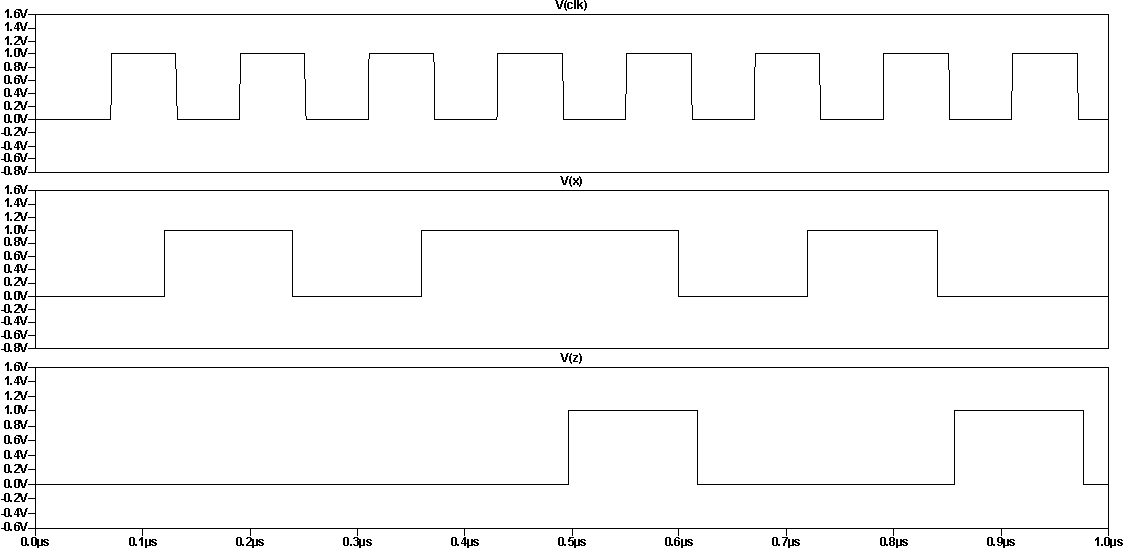
\includegraphics[width=0.9\textwidth]{inc/Q/Q12/Q12.pdf}
    \caption{LTspice Simulation Traces V(CLK), V(X) and V(Z) for Q12}\label{fig:Q11}
\end{figure}\FloatBarrier 

Figure~\ref{fig:Q11} shows the output V(Z) now producing the correct output when clocked at 120ns. Introducing a delay of 10ns, the time between a change in V(x) and the rising edge of V(CLK) now becomes $60ns + 10ns + 0.5ns= 70.5ns$, where the 10ns is the additional delay and 0.5ns, the delay caused by a 1ns rise time. the mesured value of $t_{JHBCD} = 70.36 $ which is less than 70.50ns therfore will propergate in time V(Z) to be clocked. 